\documentclass{article}

% if you need to pass options to natbib, use, e.g.:
%     \PassOptionsToPackage{numbers, compress}{natbib}
% before loading neurips_2022


% ready for submission
% \usepackage{neurips_2022}


% to compile a preprint version, e.g., for submission to arXiv, add add the
% [preprint] option:
%     \usepackage[preprint]{neurips_2022}


% to compile a camera-ready version, add the [final] option, e.g.:
\usepackage[final]{neurips_2022}


% to avoid loading the natbib package, add option nonatbib:
%    \usepackage[nonatbib]{neurips_2022}

\usepackage[utf8]{inputenc} % allow utf-8 input
\usepackage[T1]{fontenc}    % use 8-bit T1 fonts
\usepackage{hyperref}       % hyperlinks
\usepackage{url}            % simple URL typesetting
\usepackage{booktabs}       % professional-quality tables
\usepackage{amsfonts}       % blackboard math symbols
\usepackage{nicefrac}       % compact symbols for 1/2, etc.
\usepackage{microtype}      % microtypography
\usepackage{xcolor}         % colors
\usepackage{ctex}
\usepackage{graphicx}   
\usepackage{wrapfig}
\usepackage{float}
\usepackage{amsmath}
\usepackage{multirow}
\usepackage{multicol}

\bibliographystyle{unsrt}

\title{Playing Aircraft Warfare Game with Reinforcement Learning}

\author{
    Yan Zeng\\
    ShanghaiTech University\\
    \texttt{zengyan@shanghaitech.edu.cn}\\
    \AND
    Yijie Fan\\
    ShanghaiTech University\\
    \texttt{fanyj@shanghaitech.edu.cn}\\
    \AND
    Luojia Hu\\
    ShanghaiTech University\\
    \texttt{hulj@shanghaitech.edu.cn}\\
    \AND
    Ziang Li\\
    ShanghaiTech University\\
    \texttt{liza1@shanghaitech.edu.cn}\\
    \AND
    Chongyu Wang\\
    ShanghaiTech University\\
    \texttt{wangchy5@shanghaitech.edu.cn}\\    
}


\begin{document}


\maketitle

% 摘要 分数占比10%s
\begin{abstract}
    摘要没写
\end{abstract}


\section{Introduction}

    \subsection{Motivation}

    % 《经典飞机大战》是腾讯交流软件微信5.0版本在2013年8月推出的软件内置经典小游戏。
    % 该游戏的玩法十分简单,玩家只需要通过键盘上的上下左右键控制飞机移动,通过空格键发射子弹,击毁敌方飞机即可获得分数。
    % 在游戏中,玩家可以通过不断击毁敌方飞机获得分数,同时也会不断遭受敌方飞机的攻击,当玩家的血量为0时游戏结束。
    % 该游戏的玩法十分简单,但是玩家在游戏中的表现却十分复杂,这是因为游戏中的飞机是有自己的智能的,它们会根据玩家的行为做出反应。
    % 例如,当玩家的飞机靠近敌方飞机时,敌方飞机会主动向玩家的飞机发起攻击
    % 在这个project中,我们将这个游戏作为我们的仿真环境,通过强化学习的方法来训练飞机,使得飞机能够自主地在游戏中进行战斗。

    \begin{wrapfigure}{H}{7cm}
        \centering
        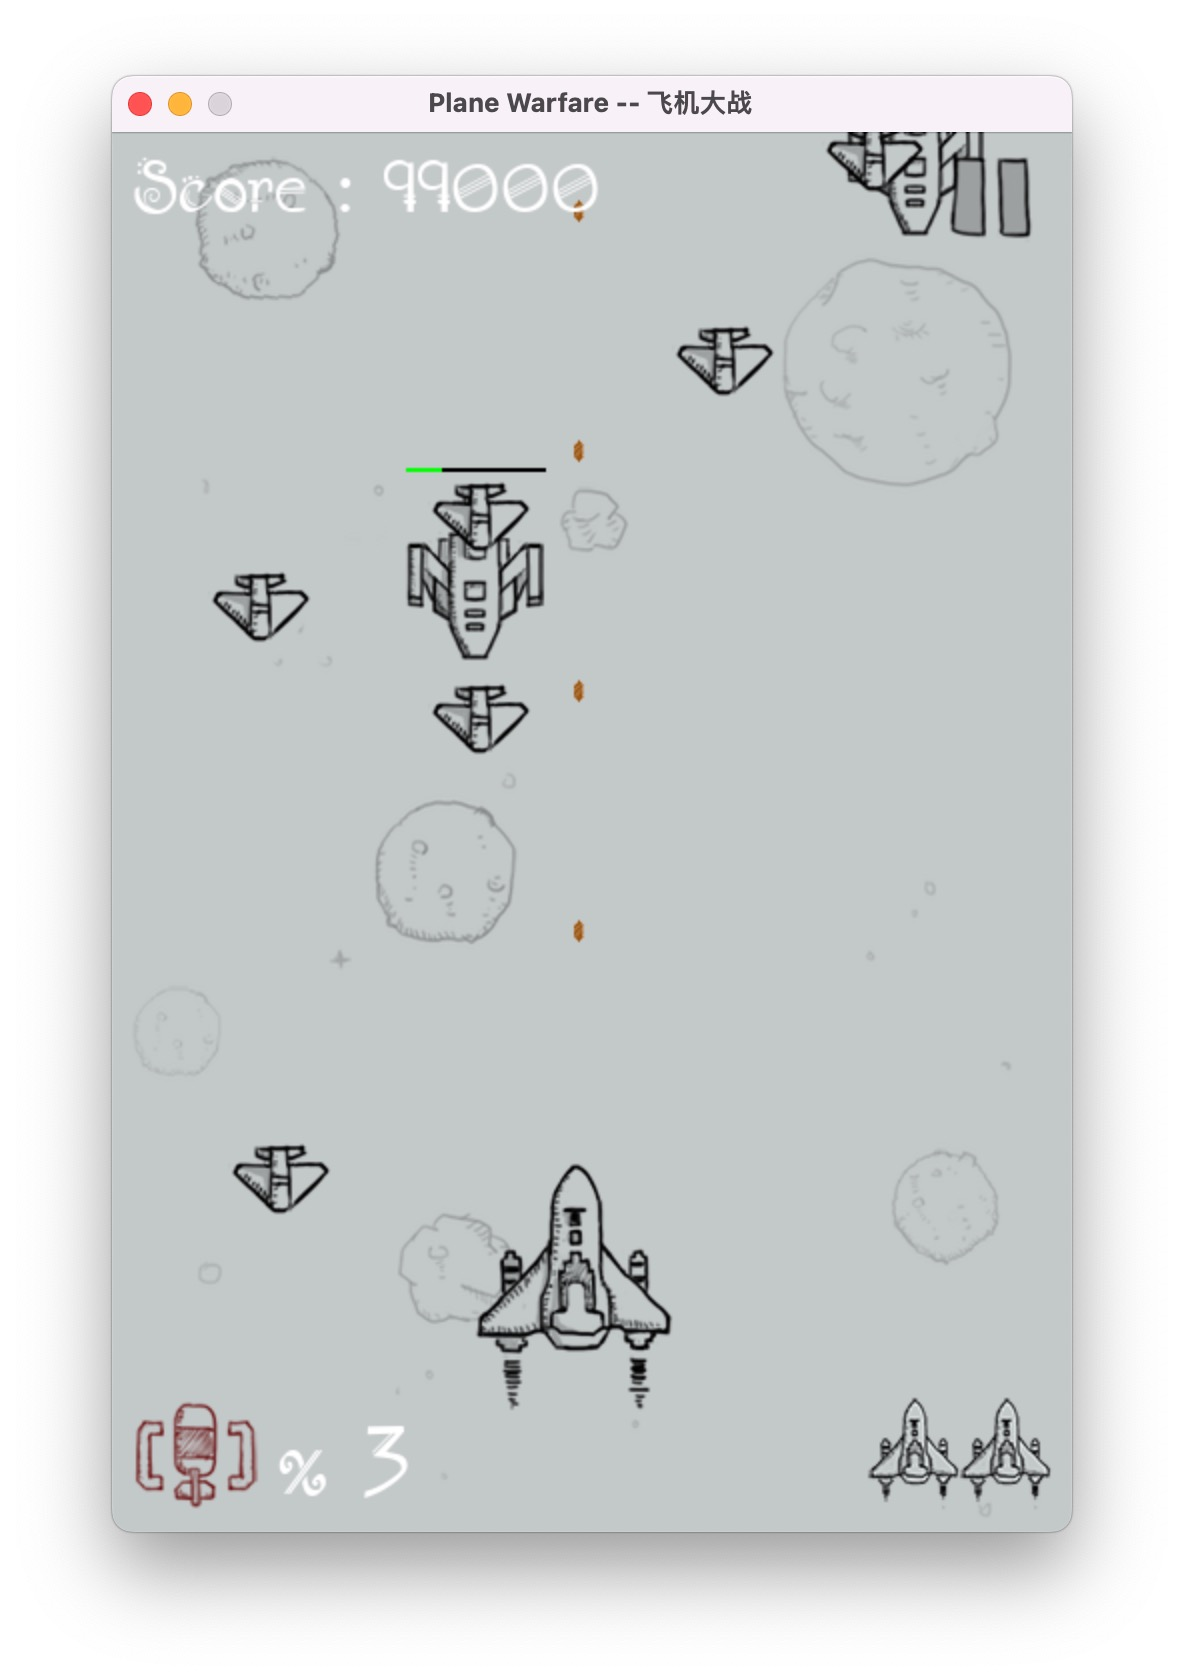
\includegraphics[width=\linewidth]{pictures/game.jpg}
        \caption{The Aircraft Warfare Game}
        \label{fig:aircraft_warfare_game}
    \end{wrapfigure}
    
    `Aircraft Warfare' is a classic game introduced in WeChat 5.0 version released in August 2013.
    The rule of the game is rather simple. In brief, players need to control the plane movement through the up, down, left and right keys on the keyboard, or shoot bullets to destroy the enemy aircraft to obtain points.
    Players can obtain points by destroying enemy aircrafts, but they may also be attacked by enemies. When the player's blood volume is 0, the game ends.
    The gameplay of the game is very simple, but the performance of the player in the game is very complex. This is because the aircraft in the game are intelligent, and they will react according to the player's behavior.
    For example, when the player's plane is close to the enemy plane, the enemy plane will actively launch an attack on the player's plane.

    In this project, we use this game as our simulation environment, and train the aircraft through the reinforcement learning method to make the aircraft autonomous in the game.

    \subsection{Aircraft Warfare game settings}

    % 在这个project中,我们使用了《经典飞机大战》的游戏规则,但是我们对游戏的设置进行了一些修改,以适应我们的强化学习算法。我们采用pygame库来实现游戏的界面,游戏的界面如图\ref{fig:aircraft_warfare_game}所示。

    In this project, we use the original rules of the `Aircraft Warfare' game, but we make some changes to the game settings to adapt to our reinforcement learning algorithm. We use the pygame library to implement the game interface, as shown in Figure \ref{fig:aircraft_warfare_game}. 

    % 在游戏中,玩家的飞机会持续发射子弹,玩家可以通过键盘上的上下左右键控制飞机移动。玩家通过空格键发射全屏子弹,能够清空屏幕中出现的所有敌机。但全屏子弹的数量具有限制。

    In the game, the player's plane will continue to fire bullets, and the player can control the plane movement through the up, down, left and right keys on the keyboard. The player can fire a full-screen bullet through the space key, which can clear all the enemy planes that appear on the screen. But the number of full-screen bullets is limited.

    % 玩家需要打中敌机来获得分数。

    % 敌机有三种类型,分别是小型敌机、中型敌机和大型敌机。小型飞机没有血量,打中一次即可消灭。中型和大型飞机都有一定的血量,打中一次会减少一定的血量,当血量为0时消灭。同时,游戏中会有血包和double bullet出现,玩家可以通过接触血包来增加生命数量,通过接触double bullet可以在接下来的一段时间内发射攻击范围更大的双倍子弹。

    The player needs to hit the enemy plane to get points.

    There are three types of enemy planes, namely small, medium and large enemy planes. Small enemies can be destroyed by a single bullet hitting. Medium and large enemies have a certain blood volume that hitting once will reduce it, and the enemy will be destroyed when the blood volume is 0. 
    
    At the same time, there will be blood bags and double bullets appearing in the game. The player can increase the number of lives by touching the blood bag, and can fire double bullets with a larger attack range in the next period of time by touching the double bullet.

\section{Model Setup}

    % 在这个project中,我们会使用approximate q-learning 来训练aircraft玩游戏。

    We will use an approximate Q-learning to train the aircraft to play the game. The approximate Q-learning algorithm is a model-free reinforcement learning algorithm, which uses a weighted sum of features to approximate the Q function. It is suitable when the state space is large. 

    \subsection{Features and Reward function}

    The features consists of mainly the position of the aircraft, enemies, and bouns (double bullet and additional life). In addition, the current status including the score, the life number remaining are also used. We will take a weighted sum of these features as the current state.

    % \subsection{Reward function}

    \subsection{Action}



\subsection{Result}

\appendix



\end{document}